\documentclass{standalone}
\usepackage{tikz}
\usetikzlibrary{patterns, positioning}
\usepackage[sfdefault]{ClearSans} %% option 'sfdefault' activates Clear Sans as the default text font
\usepackage[T1]{fontenc}

\begin{document}
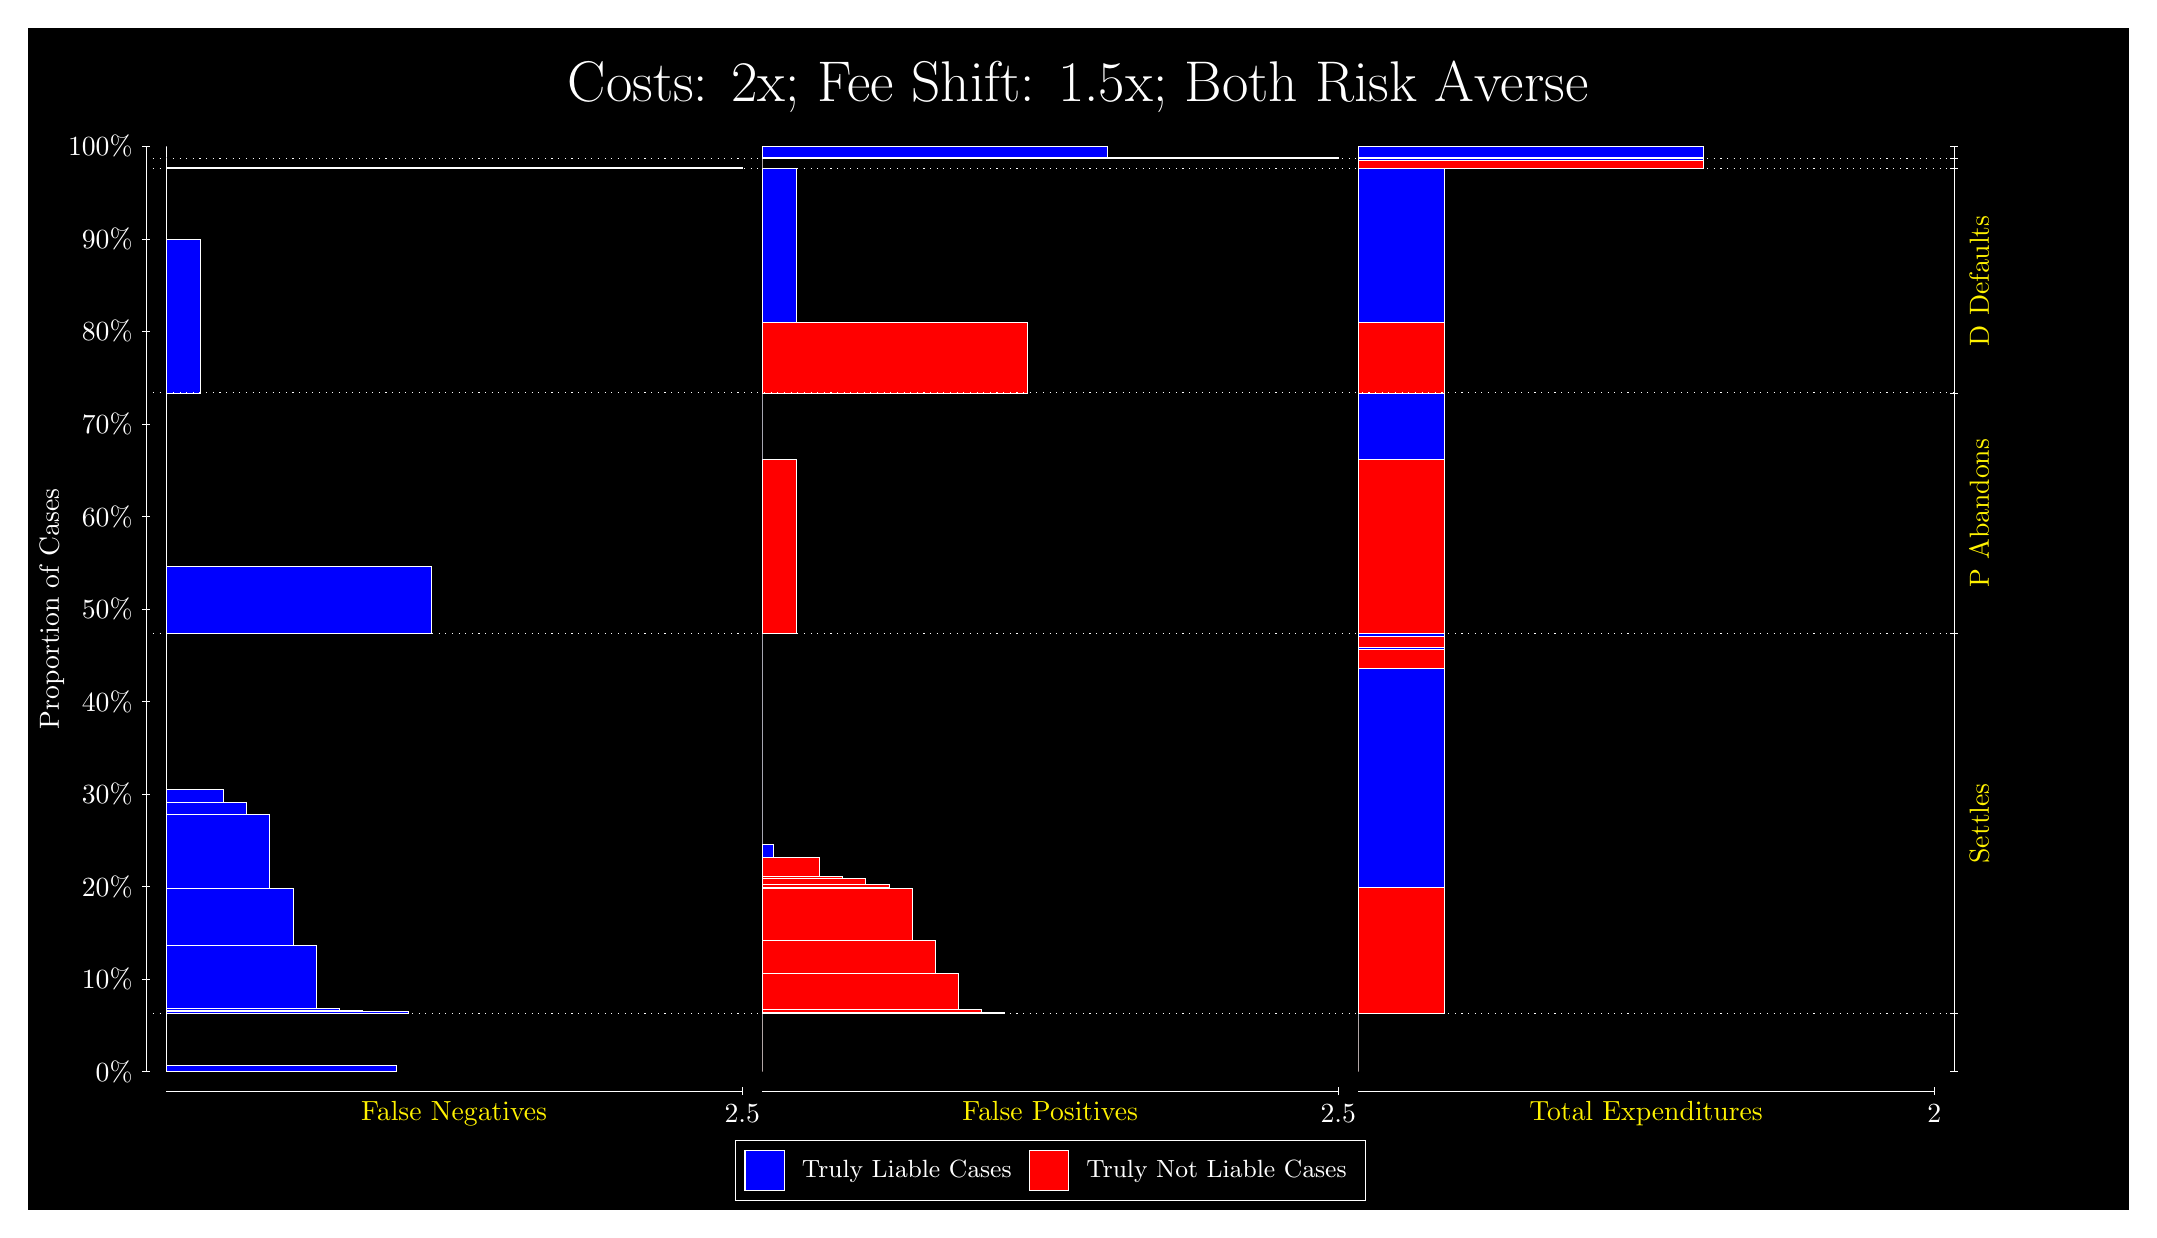
\begin{tikzpicture}
\draw[fill=black] (0,0) rectangle (26.667,15);
\draw[text=white] (0,13.5) rectangle (26.667,15) node[midway] {\huge Costs: 2x; Fee Shift: 1.5x; Both Risk Averse};
\draw[white, very thin] (1.5,1.75) -- (1.5,13.5);
\node[rotate=90, text=white, anchor=center] at (0.3, 7.625) {Proportion of Cases};
\draw[white, very thin] (1.45,1.75) -- (1.55,1.75);
\node[text=white, anchor=east] at (1.45, 1.75) {0\%};
\draw[white, very thin] (1.45,2.925) -- (1.55,2.925);
\node[text=white, anchor=east] at (1.45, 2.925) {10\%};
\draw[white, very thin] (1.45,4.1) -- (1.55,4.1);
\node[text=white, anchor=east] at (1.45, 4.1) {20\%};
\draw[white, very thin] (1.45,5.275) -- (1.55,5.275);
\node[text=white, anchor=east] at (1.45, 5.275) {30\%};
\draw[white, very thin] (1.45,6.45) -- (1.55,6.45);
\node[text=white, anchor=east] at (1.45, 6.45) {40\%};
\draw[white, very thin] (1.45,7.625) -- (1.55,7.625);
\node[text=white, anchor=east] at (1.45, 7.625) {50\%};
\draw[white, very thin] (1.45,8.8) -- (1.55,8.8);
\node[text=white, anchor=east] at (1.45, 8.8) {60\%};
\draw[white, very thin] (1.45,9.975) -- (1.55,9.975);
\node[text=white, anchor=east] at (1.45, 9.975) {70\%};
\draw[white, very thin] (1.45,11.15) -- (1.55,11.15);
\node[text=white, anchor=east] at (1.45, 11.15) {80\%};
\draw[white, very thin] (1.45,12.325) -- (1.55,12.325);
\node[text=white, anchor=east] at (1.45, 12.325) {90\%};
\draw[white, very thin] (1.45,13.5) -- (1.55,13.5);
\node[text=white, anchor=east] at (1.45, 13.5) {100\%};

\draw[white, very thin] (24.457,1.75) -- (24.457,13.5);
\draw[white, very thin] (24.407,1.75) -- (24.507,1.75);
\node[anchor=west] at (24.407, 1.75) {};
\draw[white, very thin] (24.407,2.4922) -- (24.507,2.4922);
\node[anchor=west] at (24.407, 2.4922) {};
\draw[white, very thin] (24.407,7.312) -- (24.507,7.312);
\node[anchor=west] at (24.407, 7.312) {};
\draw[white, very thin] (24.407,10.37) -- (24.507,10.37);
\node[anchor=west] at (24.407, 10.37) {};
\draw[white, very thin] (24.407,13.217) -- (24.507,13.217);
\node[anchor=west] at (24.407, 13.217) {};
\draw[white, very thin] (24.407,13.342) -- (24.507,13.342);
\node[anchor=west] at (24.407, 13.342) {};
\draw[white, very thin] (24.407,13.5) -- (24.507,13.5);
\node[anchor=west] at (24.407, 13.5) {};

\draw[white, very thin, fill=blue] (1.75,1.75) rectangle (4.6775,1.8281);
\draw[white, very thin, fill=red] (1.75,1.8281) rectangle (1.75,2.4922);
\draw[white, very thin, fill=blue] (1.75,2.4922) rectangle (4.8239,2.512);
\draw[white, very thin, fill=blue] (1.75,2.512) rectangle (4.5312,2.5137);
\draw[white, very thin, fill=blue] (1.75,2.5137) rectangle (4.2384,2.5322);
\draw[white, very thin, fill=blue] (1.75,2.5322) rectangle (3.9457,2.5518);
\draw[white, very thin, fill=blue] (1.75,2.5518) rectangle (3.6529,3.3513);
\draw[white, very thin, fill=blue] (1.75,3.3513) rectangle (3.3602,4.073);
\draw[white, very thin, fill=blue] (1.75,4.073) rectangle (3.0674,5.0178);
\draw[white, very thin, fill=blue] (1.75,5.0178) rectangle (2.7746,5.1642);
\draw[white, very thin, fill=blue] (1.75,5.1642) rectangle (2.4819,5.3367);
\draw[white, very thin, fill=red] (1.75,5.3367) rectangle (1.75,7.312);
\draw[white, very thin, fill=blue] (1.75,7.312) rectangle (5.1167,8.1606);
\draw[white, very thin, fill=red] (1.75,8.1606) rectangle (1.75,10.37);
\draw[white, very thin, fill=blue] (1.75,10.37) rectangle (2.1891,12.316);
\draw[white, very thin, fill=red] (1.75,12.316) rectangle (1.75,13.217);
\draw[white, very thin, fill=blue] (1.75,13.217) rectangle (9.0689,13.235);
\draw[white, very thin, fill=red] (1.75,13.235) rectangle (1.75,13.342);
\draw[white, very thin, fill=red] (1.75,13.342) rectangle (1.75,13.361);
\draw[white, very thin, fill=blue] (1.75,13.361) rectangle (1.75,13.5);
\draw[white, very thin, fill=red] (9.3189,1.75) rectangle (9.3189,2.4141);
\draw[white, very thin, fill=blue] (9.3189,2.4141) rectangle (9.3189,2.4922);
\draw[white, very thin, fill=red] (9.3189,2.4922) rectangle (12.393,2.5046);
\draw[white, very thin, fill=red] (9.3189,2.5046) rectangle (12.1,2.5366);
\draw[white, very thin, fill=red] (9.3189,2.5366) rectangle (11.807,2.9976);
\draw[white, very thin, fill=red] (9.3189,2.9976) rectangle (11.515,3.417);
\draw[white, very thin, fill=red] (9.3189,3.417) rectangle (11.222,4.0749);
\draw[white, very thin, fill=red] (9.3189,4.0749) rectangle (10.929,4.0851);
\draw[white, very thin, fill=red] (9.3189,4.0851) rectangle (10.929,4.124);
\draw[white, very thin, fill=red] (9.3189,4.124) rectangle (10.636,4.2085);
\draw[white, very thin, fill=red] (9.3189,4.2085) rectangle (10.344,4.2284);
\draw[white, very thin, fill=red] (9.3189,4.2284) rectangle (10.051,4.4675);
\draw[white, very thin, fill=blue] (9.3189,4.4675) rectangle (9.4652,4.6401);
\draw[white, very thin, fill=blue] (9.3189,4.6401) rectangle (9.3189,7.312);
\draw[white, very thin, fill=red] (9.3189,7.312) rectangle (9.758,9.5211);
\draw[white, very thin, fill=blue] (9.3189,9.5211) rectangle (9.3189,10.37);
\draw[white, very thin, fill=red] (9.3189,10.37) rectangle (12.686,11.27);
\draw[white, very thin, fill=blue] (9.3189,11.27) rectangle (9.758,13.217);
\draw[white, very thin, fill=red] (9.3189,13.217) rectangle (9.3189,13.324);
\draw[white, very thin, fill=blue] (9.3189,13.324) rectangle (9.3189,13.342);
\draw[white, very thin, fill=red] (9.3189,13.342) rectangle (16.638,13.361);
\draw[white, very thin, fill=blue] (9.3189,13.361) rectangle (13.71,13.5);
\draw[white, very thin, fill=red] (16.888,1.75) rectangle (16.888,2.4141);
\draw[white, very thin, fill=blue] (16.888,2.4141) rectangle (16.888,2.4922);
\draw[white, very thin, fill=red] (16.888,2.4922) rectangle (17.986,4.0851);
\draw[white, very thin, fill=blue] (16.888,4.0851) rectangle (17.986,6.8763);
\draw[white, very thin, fill=red] (16.888,6.8763) rectangle (17.986,7.1154);
\draw[white, very thin, fill=blue] (16.888,7.1154) rectangle (17.986,7.1352);
\draw[white, very thin, fill=red] (16.888,7.1352) rectangle (17.986,7.2785);
\draw[white, very thin, fill=blue] (16.888,7.2785) rectangle (17.986,7.312);
\draw[white, very thin, fill=red] (16.888,7.312) rectangle (17.986,9.5211);
\draw[white, very thin, fill=blue] (16.888,9.5211) rectangle (17.986,10.37);
\draw[white, very thin, fill=red] (16.888,10.37) rectangle (17.986,11.27);
\draw[white, very thin, fill=blue] (16.888,11.27) rectangle (17.986,13.217);
\draw[white, very thin, fill=red] (16.888,13.217) rectangle (21.279,13.324);
\draw[white, very thin, fill=blue] (16.888,13.324) rectangle (21.279,13.342);
\draw[white, very thin, fill=red] (16.888,13.342) rectangle (21.279,13.361);
\draw[white, very thin, fill=blue] (16.888,13.361) rectangle (21.279,13.5);
\draw[white, dotted] (1.5,2.4922) -- (24.457,2.4922);
\draw[white, dotted] (1.5,7.312) -- (24.457,7.312);
\draw[white, dotted] (1.5,10.37) -- (24.457,10.37);
\draw[white, dotted] (1.5,13.217) -- (24.457,13.217);
\draw[white, dotted] (1.5,13.342) -- (24.457,13.342);
\draw[white, very thin] (1.75,1.5) -- (9.0689,1.5);
\node[text=yellow, anchor=north] at (5.4094, 1.5) {False Negatives};
\draw[white, very thin] (9.0689,1.45) -- (9.0689,1.55);
\node[text=white, anchor=north] at (9.0689, 1.45) {2.5};

\draw[white, very thin] (9.3189,1.5) -- (16.638,1.5);
\node[text=yellow, anchor=north] at (12.978, 1.5) {False Positives};
\draw[white, very thin] (16.638,1.45) -- (16.638,1.55);
\node[text=white, anchor=north] at (16.638, 1.45) {2.5};

\draw[white, very thin] (16.888,1.5) -- (24.207,1.5);
\node[text=yellow, anchor=north] at (20.547, 1.5) {Total Expenditures};
\draw[white, very thin] (24.207,1.45) -- (24.207,1.55);
\node[text=white, anchor=north] at (24.207, 1.45) {2};


\node[text=yellow, centered, rotate=90] at (24.777, 4.9021) {Settles};
\node[text=yellow, centered, rotate=90] at (24.777, 8.8408) {P Abandons};
\node[text=yellow, centered, rotate=90] at (24.777, 11.793) {D Defaults};



\draw (12.978300999999998,1.5) node[draw=none] (baseCoordinate) {};
\begin{scope}[align=center]
        \matrix[scale=0.5, draw=white, below=0.5cm of baseCoordinate, nodes={draw}, column sep=0.1cm]{
            \node[rectangle, draw, minimum width=0.5cm, minimum height=0.5cm, fill=blue] {}; &
            \node[draw=none, font=\small, text=white] (B) {Truly Liable Cases}; &
            \node[rectangle, draw, minimum width=0.5cm, minimum height=0.5cm, fill=red] {}; &
            \node[draw=none, font=\small, text=white] (B) {Truly Not Liable Cases}; \\
            };
\end{scope}

\end{tikzpicture}
\end{document}